\documentclass[11pt]{ctexart}
\usepackage{a4}
\usepackage{graphicx}
\usepackage{geometry}
\usepackage{amsmath}
\usepackage{mathtools}
\geometry{a4paper,left=2cm,right=2cm,top=2.5cm,bottom=2.5cm}

\title{几何基础作业4}
\author{无名}
\date{\today}

\begin{document}
\maketitle
\section{尺规作图正五边形}
\begin{figure}[htb]
    \begin{center}
        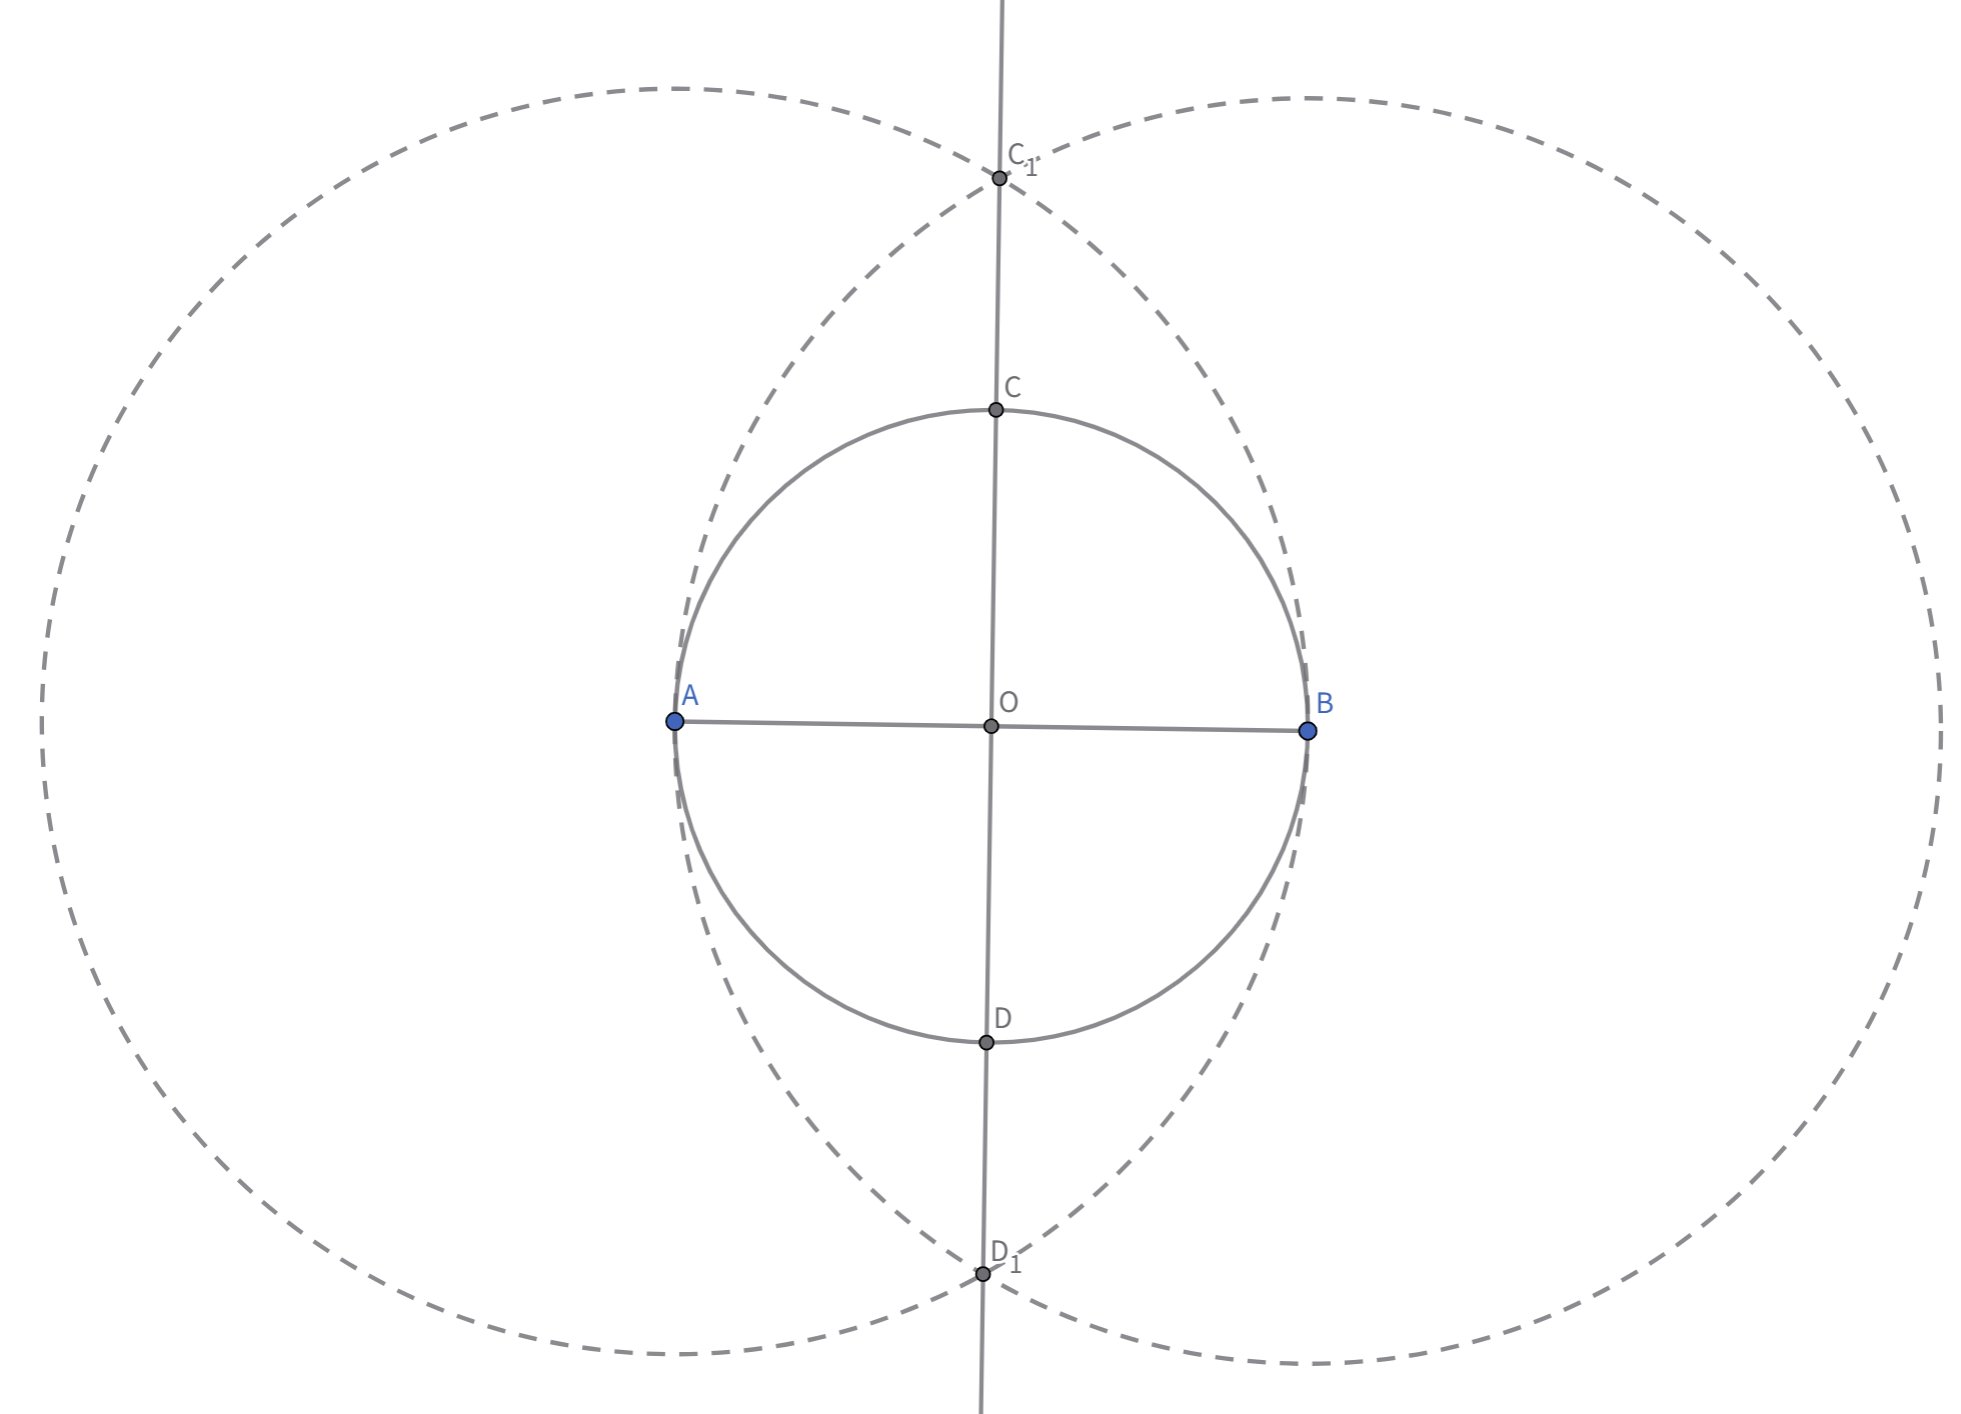
\includegraphics[width=0.7\linewidth]{1.png}
        \caption{}
    \end{center}
\end{figure}

如图1，我们有线段$AB$，现在以A,B为圆心，以$AB$为半径画圆，交于$C_1,C_2$两点，连接$C_1C_2$做直线即为$AB$的中垂线，记其与$AB$的交点为O。

以O为圆心，$AB$为半径画圆，交$C_1C_2$于$C,D$
\newpage
\begin{figure}[htb]
    \begin{center}
        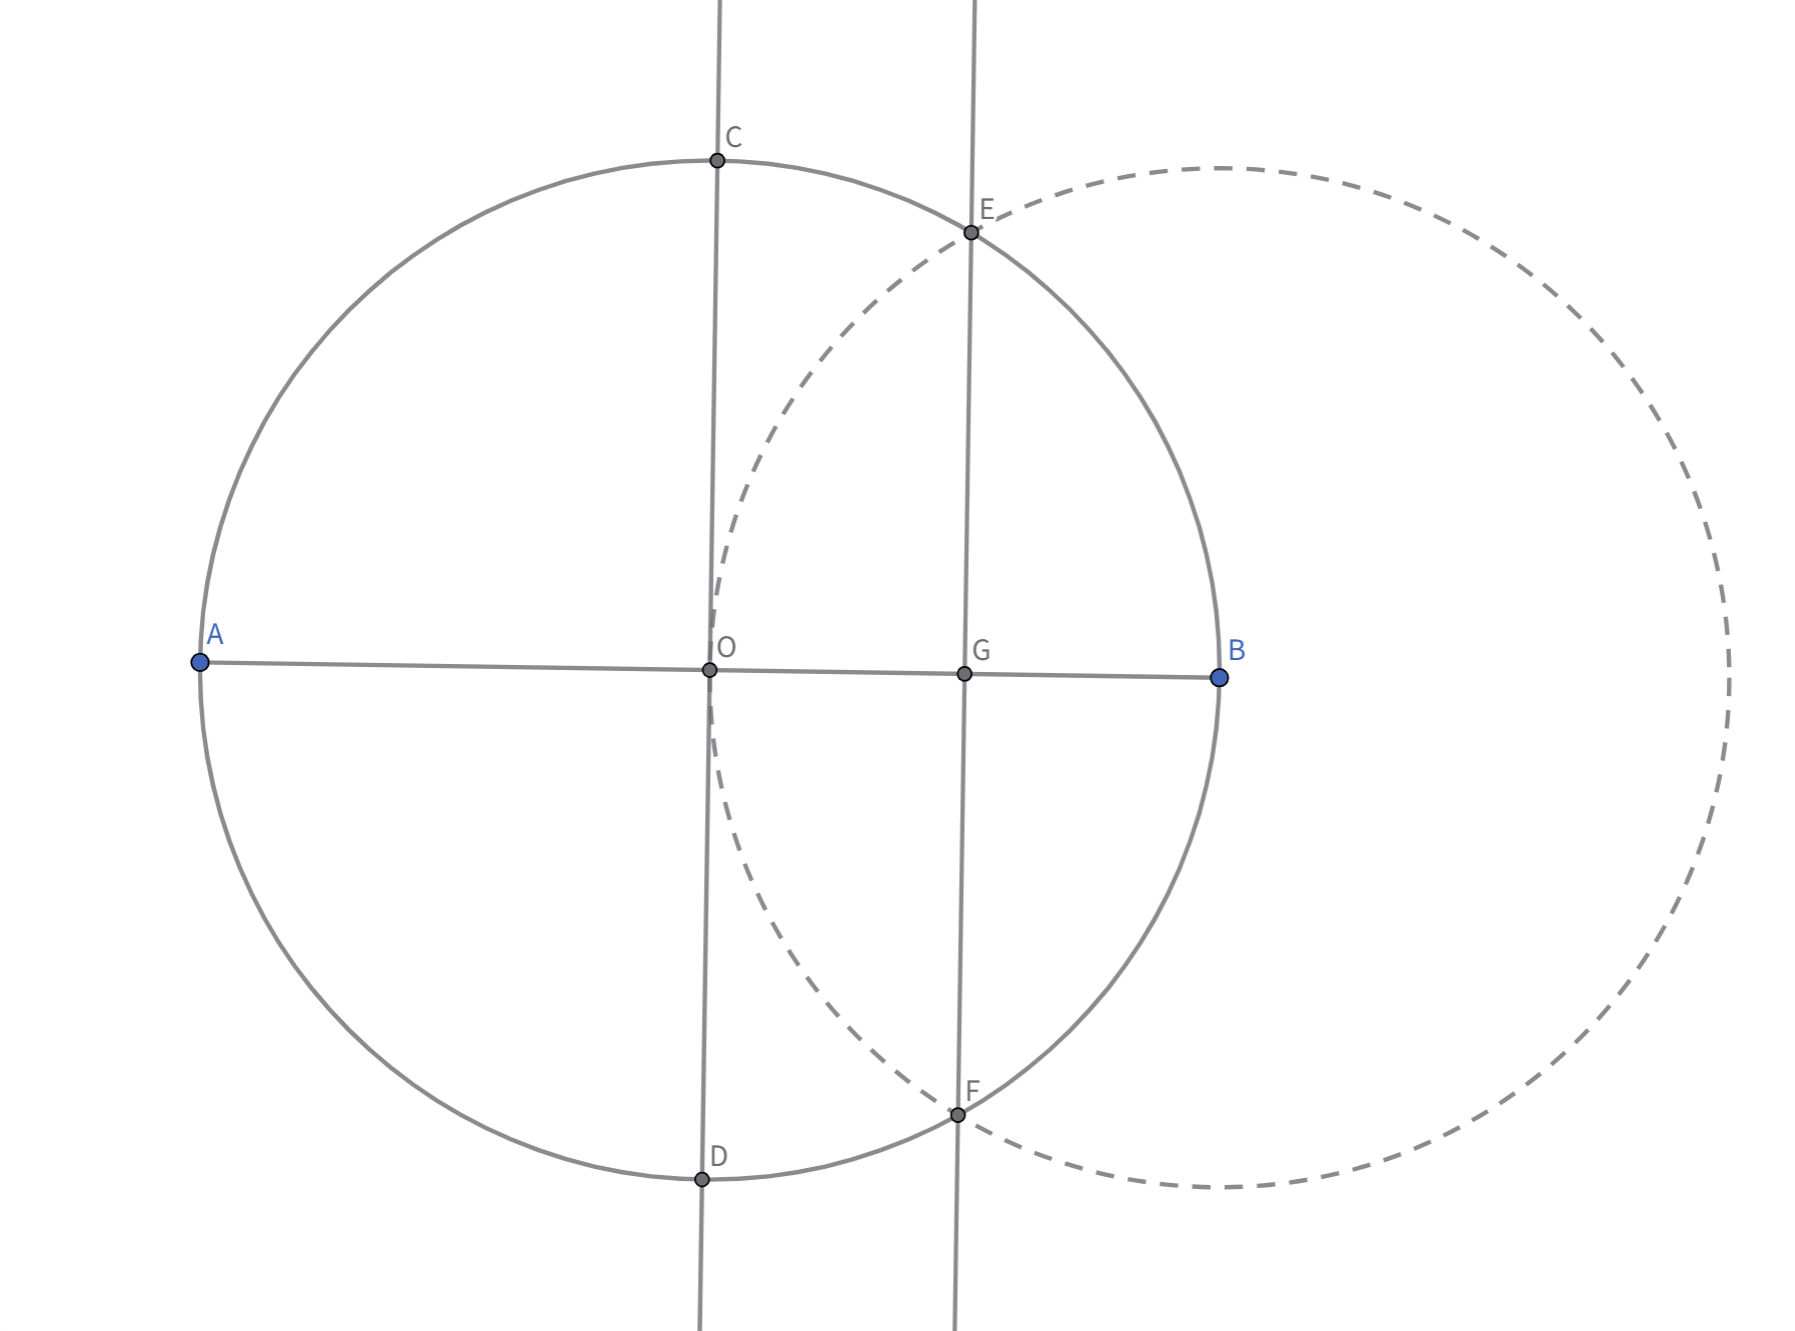
\includegraphics[width=0.6\linewidth]{2.png}
        \caption{}
    \end{center}
\end{figure}

如图2，以B为圆心，OB为半径画圆，交圆O于E,F两点，连接EF交AB于G，则EF就是OB的中垂线。

\begin{figure}[htb]
    \begin{center}
        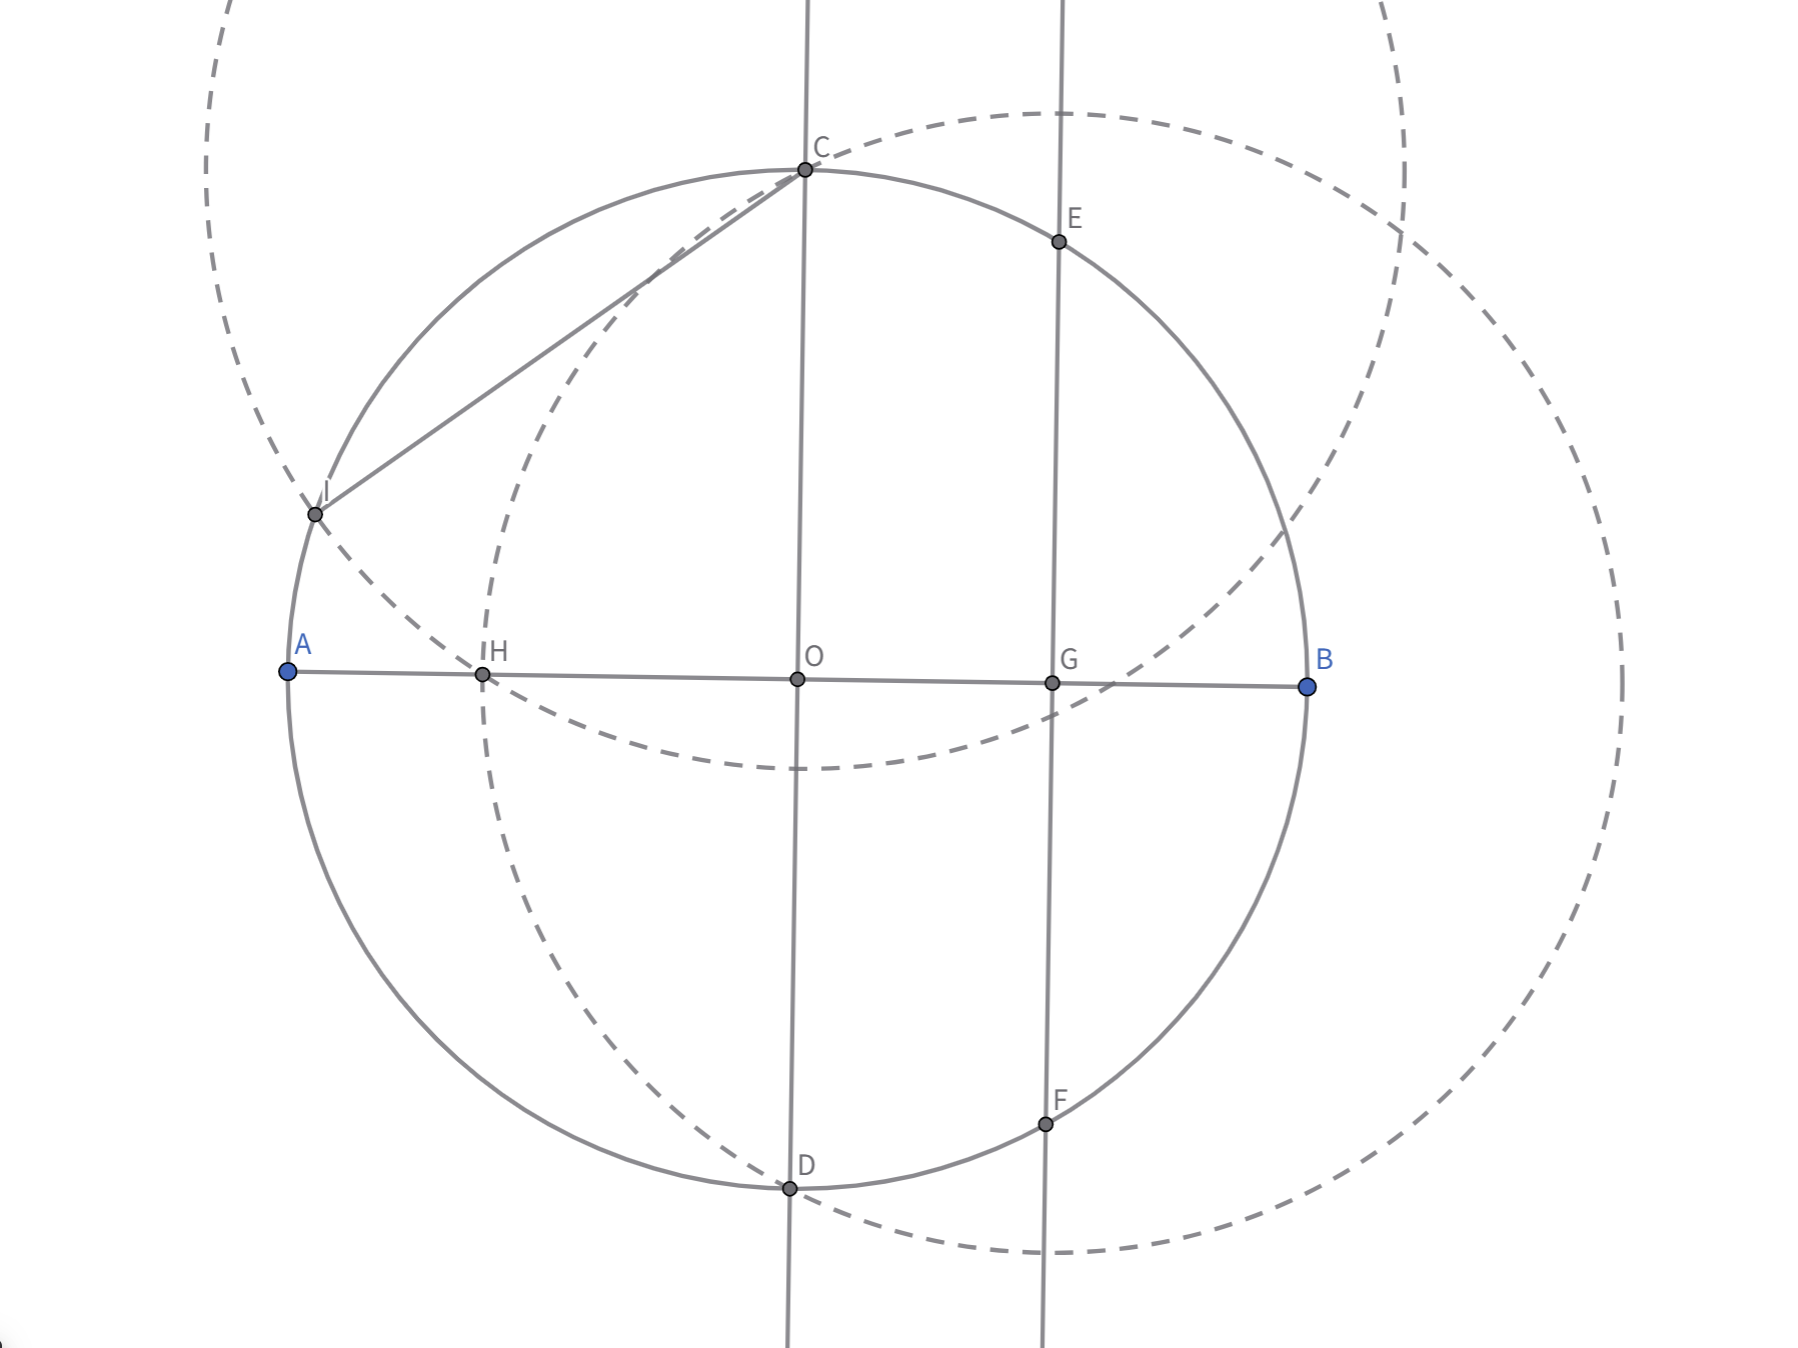
\includegraphics[width=0.6\linewidth]{3.png}
        \caption{}
    \end{center}
\end{figure}

如图3，以G为圆心，GC为半径做圆，交AB于H，再以C为圆心，CH为半径画弧，交圆O于I点。此时CI就是所画正五边形的边。
\newpage
\begin{figure}[htb]
    \begin{center}
        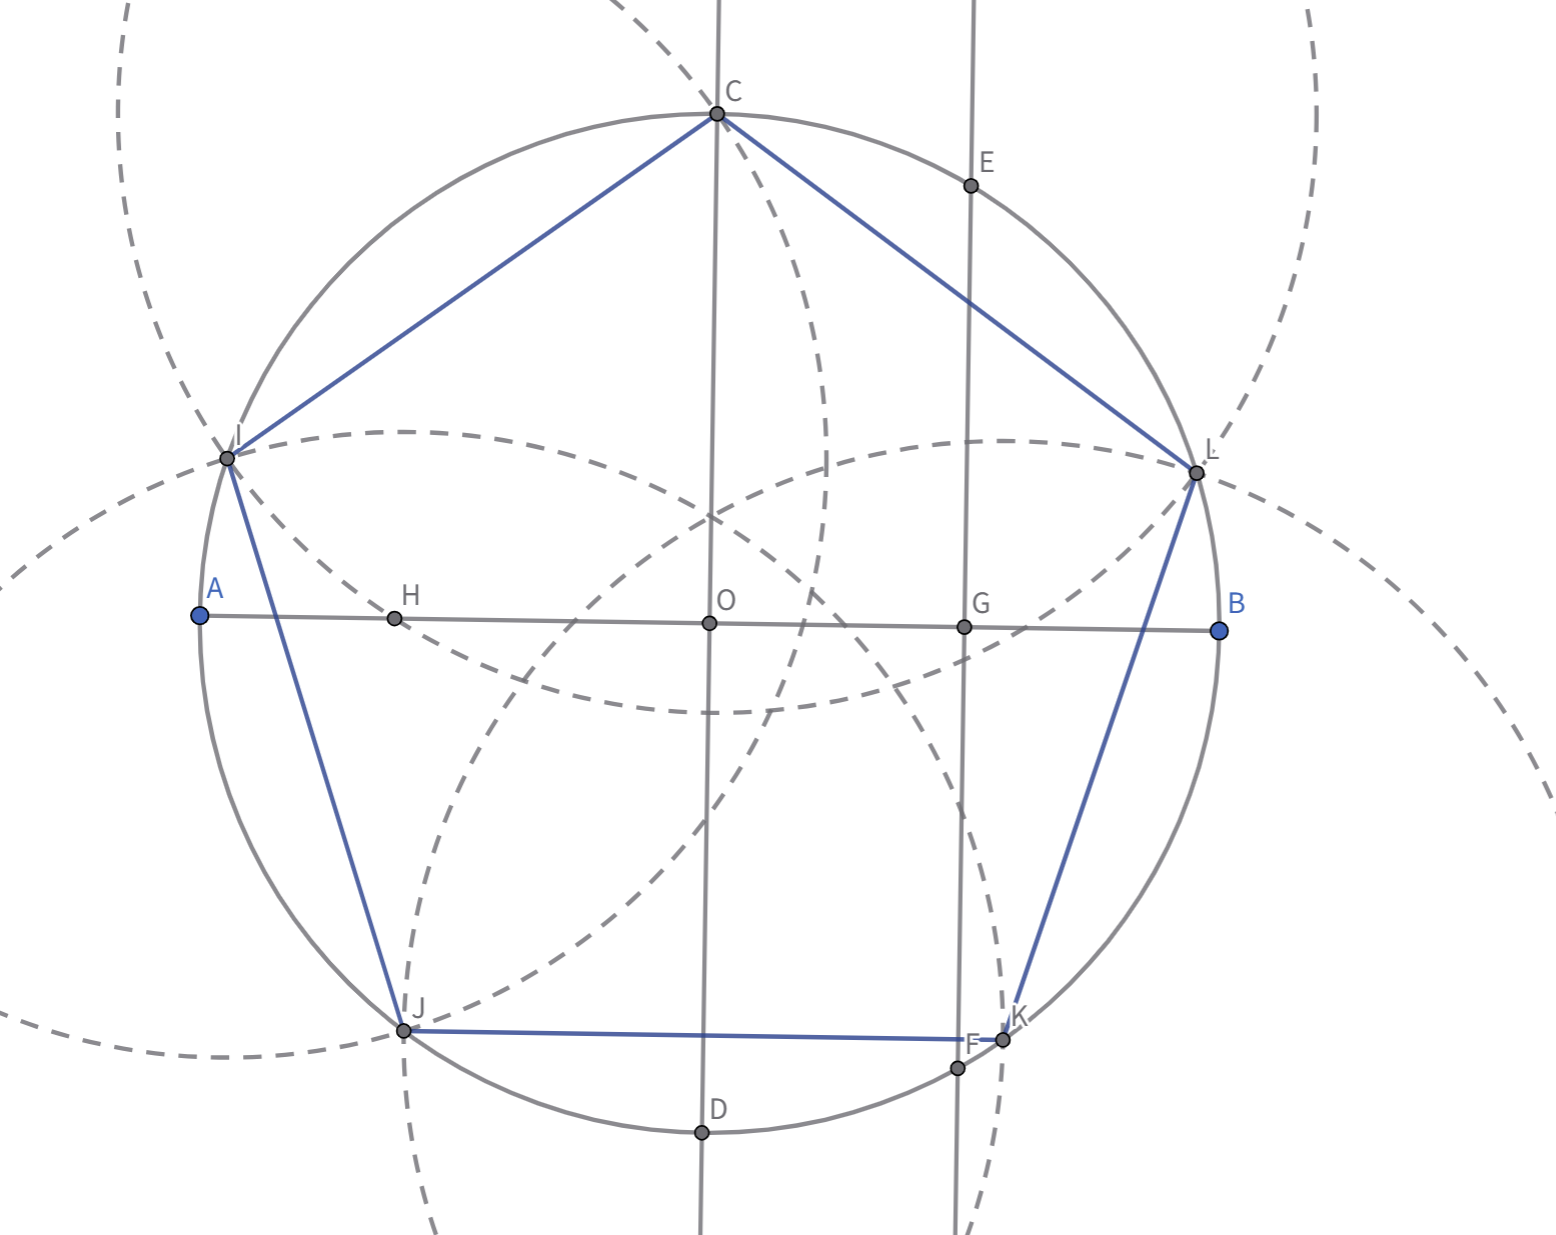
\includegraphics[width=0.6\linewidth]{4.png}
        \caption{}
    \end{center}
\end{figure}

如图4，以为CI为半径画圆补全正五边形的边，即得到所画图形。

\section{尺规作图正十五边形}

\begin{figure}[htb]
    \begin{center}
        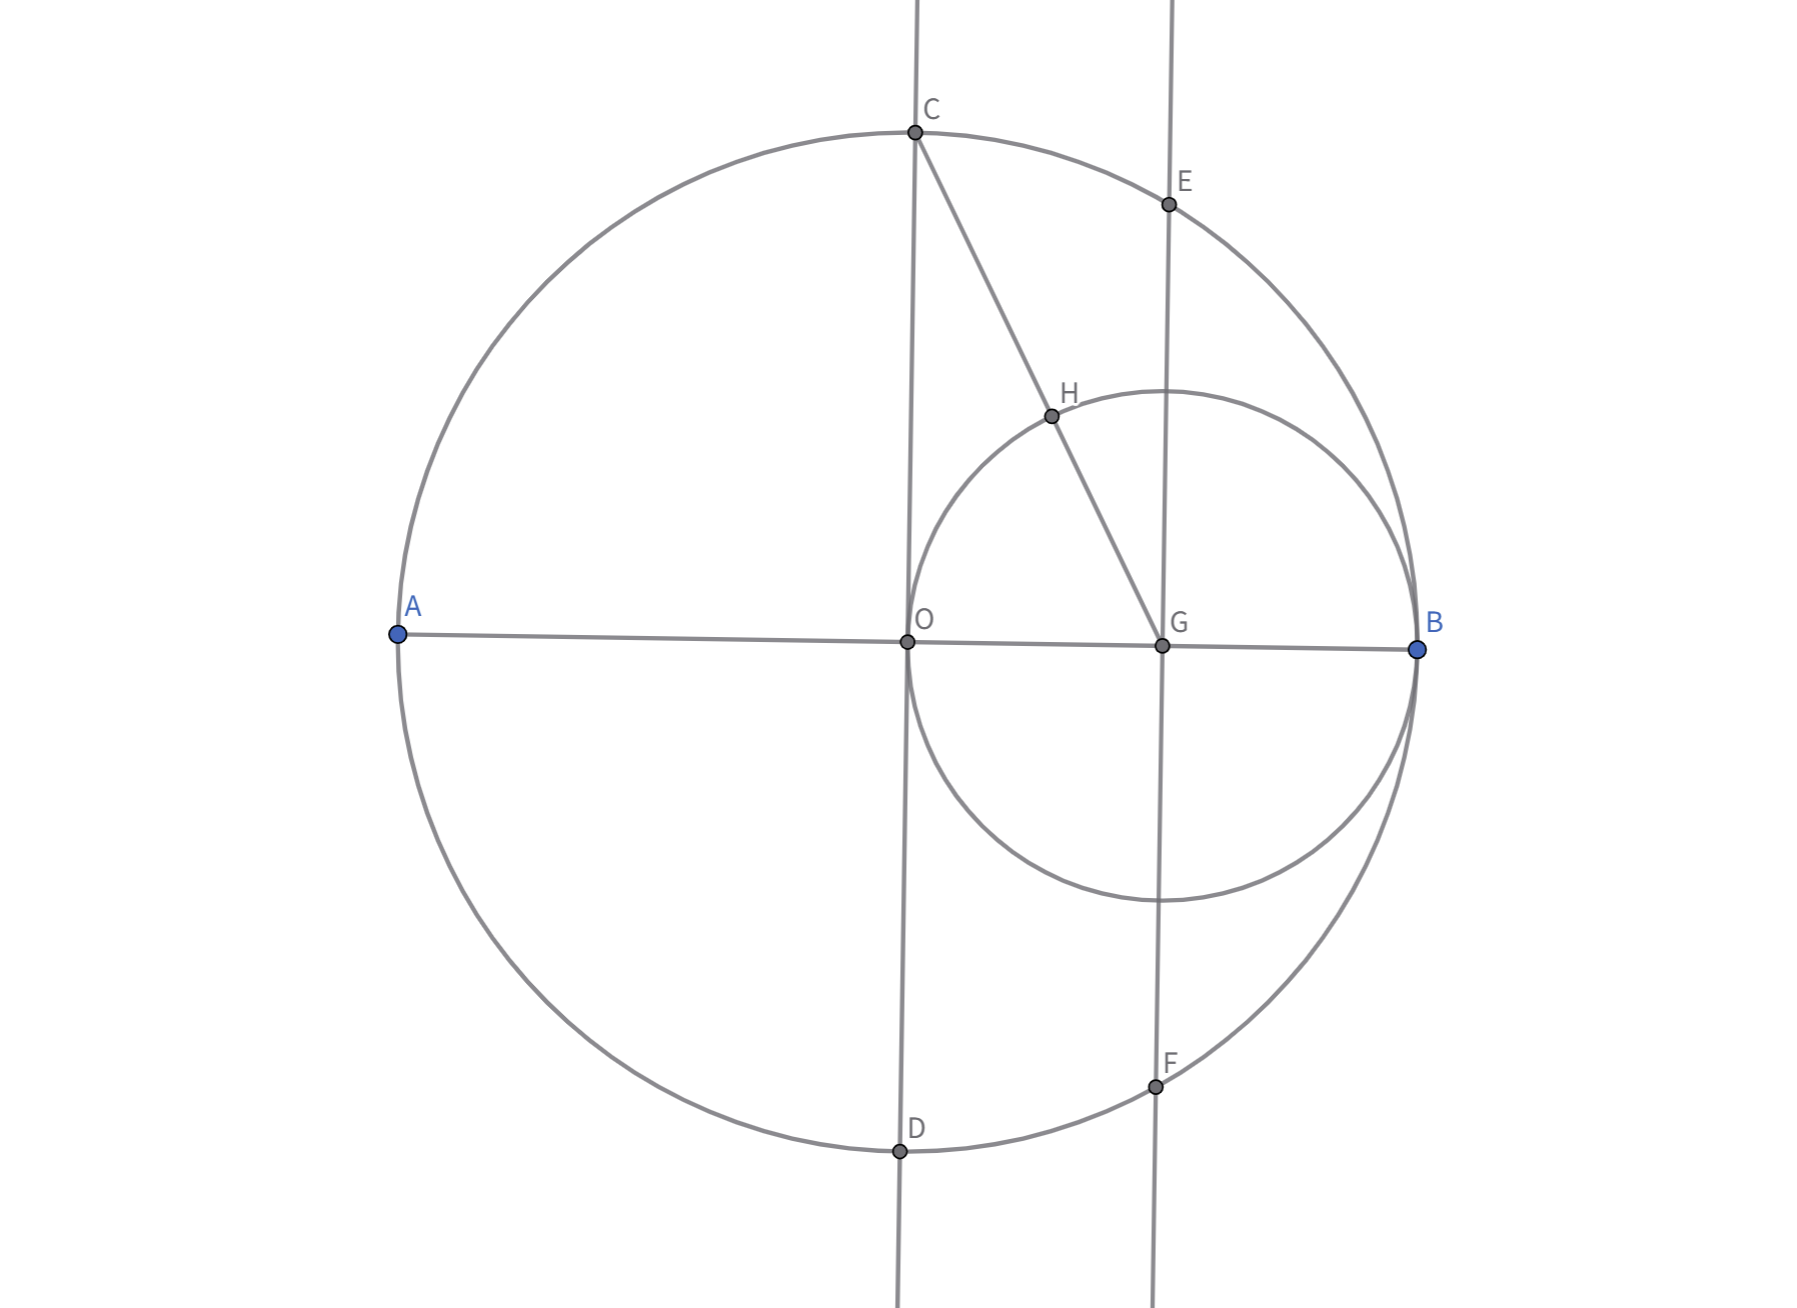
\includegraphics[width=0.6\linewidth]{5.png}
        \caption{}
    \end{center}
\end{figure}

如图5，在图2的基础上连接CG，以G为圆心，OG为半径做圆，交CG线段于H。
\newpage
\begin{figure}[htb]
    \begin{center}
        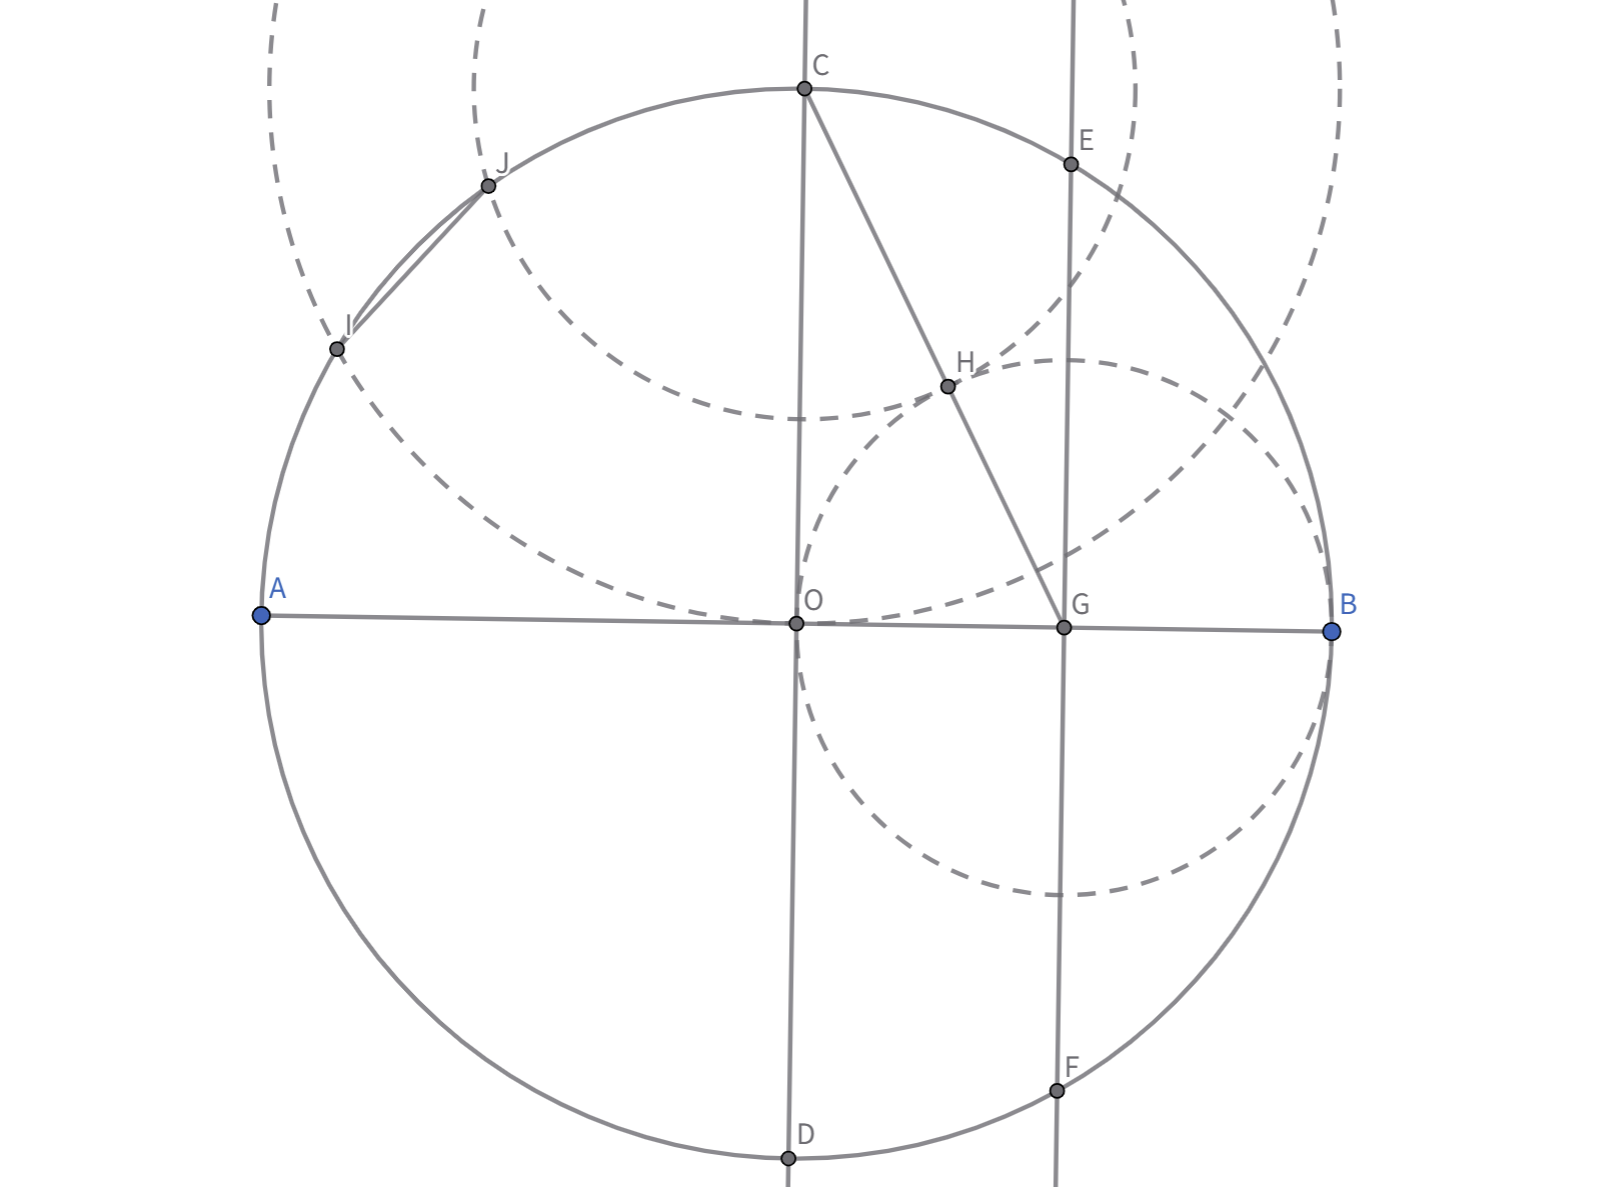
\includegraphics[width=0.6\linewidth]{6.png}
        \caption{}
    \end{center}
\end{figure}

如图6，以C为圆心，CO,CH为半径做圆，如图分别交圆O于I,J两点。

此时IJ即为正十五边形的一边。

\begin{figure}[htb]
    \begin{center}
        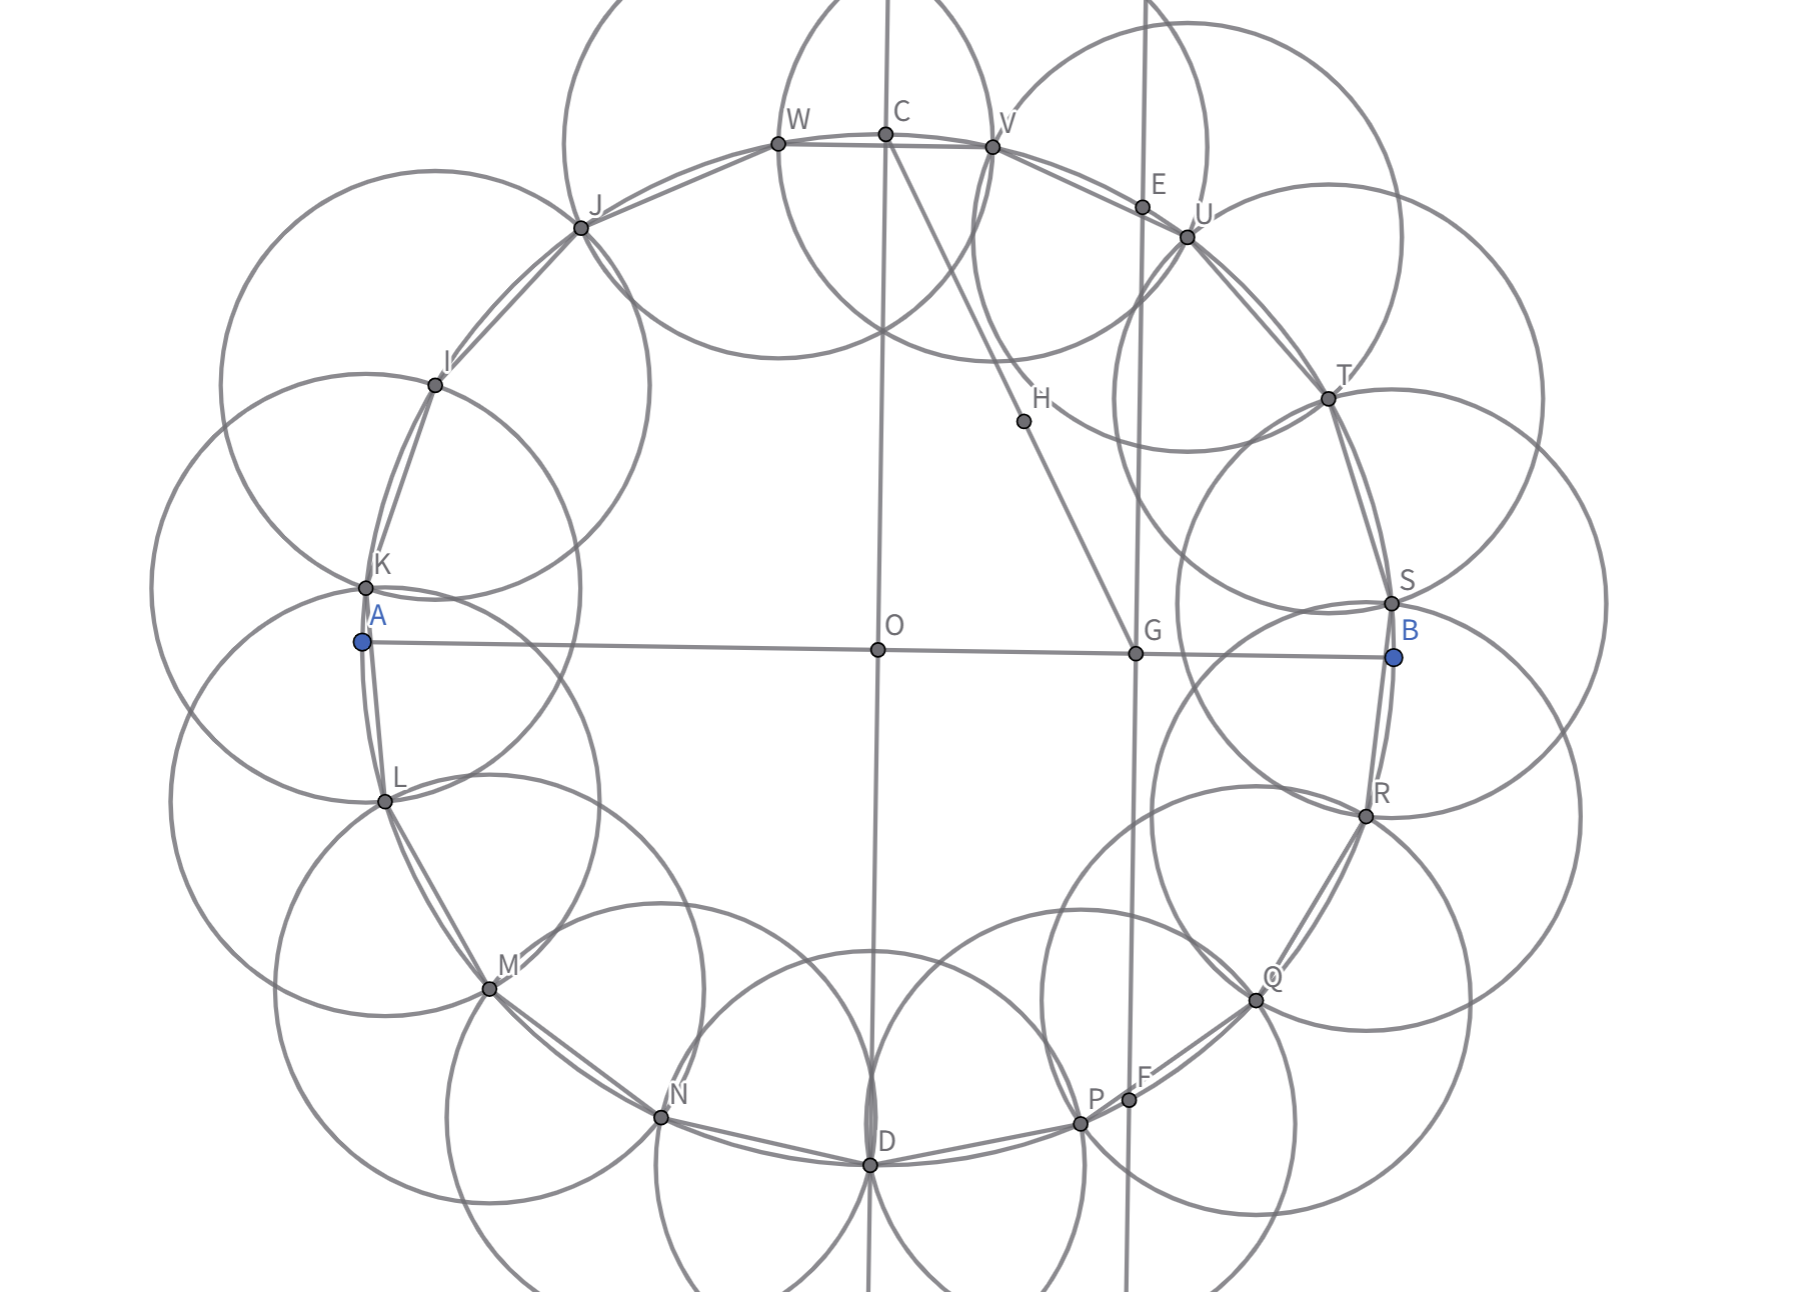
\includegraphics[width=0.6\linewidth]{7.png}
        \caption{}
    \end{center}
\end{figure}

如图7，以IJ为半径画圆补全，即得到正十五边形。

\newpage
\section{用正余弦定理推导海伦公式}
\subsection{海伦公式}
已知$\bigtriangleup ABC$,角$A,B,C$的对边分别为$a,b,c$，那么$p=\frac{a+b+c}{2}$
\[S_{\bigtriangleup ABC}=\sqrt{p(p-a)(p-b)(p-c)} 
\]
\subsection{证明}
由正弦定理，
\[S_{\bigtriangleup ABC }=\frac{1}{2}ab\sin C\]

\[\cos^2 C+\sin^2 C=1\]

那么
\[S_{\bigtriangleup ABC }=\frac{1}{2}ab \sqrt{1-\cos^2 C}\]

由余弦定理，$\cos C=\frac{a^2+b^2-c^2}{2ab}$,那么

\[\cos^2 C=\frac{(a^2+b^2-c^2)^2}{4a^2b^2}=\frac{a^4+b^4+c^4+2a^2b^2-2a^2c^2-2b^2c^2}{4a^2b^2}\]

\[1-\cos^2 C=\frac{2a^2b^2+2a^2c^2+2b^2c^2-a^4-b^4-c^4}{4a^2b^2}\]

\[\sqrt{1-\cos^2 C}=\frac{\sqrt{2a^2b^2+2a^2c^2+2b^2c^2-a^4-b^4-c^4}}{2ab}\]

那么
\[
\begin{split}
S_{\bigtriangleup ABC }&=\frac{1}{4}\sqrt{2a^2b^2+2a^2c^2+2b^2c^2-a^4-b^4-c^4}\\
&=\sqrt{\frac{(a+b+c)(b+c-a)(a+c-b)(a+b-c)}{16}}\\
&=\sqrt{p(p-a)(p-b)(p-c)}\\
\end{split} 
\]

证毕
\end{document}